% ---------------------------------------------------------------------------
\subsection{Computational Challenges}

Most advances in high-performance computing have focused on the scale,
performance and optimization of single long simulations. However, due to the
end of Dennard scaling and methodological advances, many applications are now
formulated using multiple, shorter ensemble-based simulations. Yet, there are
limited software solutions that can execute scalable heterogeneous
computational tasks. Furthermore, statistically meaningful results derived
from simulations are of critical interest, as they can leverage additional
sampling of simulations which could lead to an improvement in precision 
of free energy calculations. Such decisions typically, cannot be made {\it a
priori} and require postmortem user intervention in order to analyze and spawn
additional simulations.

% To encode an algorithm into a set of tasks requires a workflow system that
% exposes an interface to describe tasks, dependencies, and an execution
% pattern. Once the algorithm is encoded into a set of tasks, the workflow
% system is required to translate tasks into executables, coordinate task
% dependencies, and acquire and manage resources.

%\jhanote{I'm changing the order of paragraphs: promoting adaptivity, as we
%seem to be building the case for decision making.}

% We define \textbf{adaptivity} as the ability to revisit a prior execution
% decision based on a runtime evaluation. Adapting workflows at runtime requires
% incorporating additional parallelism, redistributing of resources across
% tasks, and analyzing the performance and functionality of added adaptivity to
% evaluate its benefits and further design.

Many workflow management can be used to automate ensemble-based workflows but
suffer of several limitations. Among these, two of the most relevant are long
time to adoption and lack of dynamic capabilities.
% monolithic designs provide end-to-end capabilities to execute workflows on
% heterogeneous and distributed cyberinfrastructure. Other workflow systems
% entail
Workflow system with featureful but complex interface models impose
substantial overhead when integrating application workflows in the runtime
system, preventing users from quick and flexible applications prototyping.
Moreover, any intervention during runtime such as spawning additional 
simulations could require a redistribution of resources.  
% Furthermore, performance and resource utilization are necessary to ensure
% scalability of tasks, with minimal overhead in scheduling.
Current workflow management systems do not provide adequate
support for dynamic resource utilization, limiting the possibility to modify 
workflow models at runtime. 

% ---------------------------------------------------------------------------
\subsection{HTBAC}

In response to these challenges and requirements, and the absence of
middleware providing scalability and generality to applications for ensemble-
based protocols executed on HPC, we discuss the design and implementation of
HTBAC, which builds upon the RADICAL-Cybertools (RCT), a set of software
building blocks that eschew monolithic workloads. RCT is engineered to scale
across diverse computing platforms with the rapid ability to design a
multitude of workflows. HTBAC promotes biosimulation protocols to high-level
programming abstractions to enable the user to specify and efficiently grow
protocols, thereby enabling concurrent screening of drug candidates with the
added functionality to guide simulations in real-time.


Efficient execution of binding affinity calculation protocols on different
cyberinfrastructure poses several technical challenges, none of which are of
interest to domain scientists. This suggests three requirements for HTBAC\@:
(1) enabling the execution of multiple protocols on heterogeneous
cyberinfrastructure; (2) abstract the complexity of building protocols,
execution and resource management from the user; and (3) providing adaptive
features to enables changes to the workflow, i.e. the task-graph during
runtime, based on decisions generated by previous tasks.

%\jhanote{NEED DIAGRAMS ASAP}

% ---------------------------------------------------------------------------
\subsection{Implementation}

In section \ref{sec:science-drivers}, we described two examples of ensemble-based protocols (ESMACS/TIES)
where each protocol contains multiple simulation steps followed by multiple 
aggregate statistical analysis steps. Steps vary in data input dependencies, 
computational resource requirements and MD execution engines. We define 
each step as a computational \textbf{task} and the aggregation of these 
steps alongside their dependencies as a \textbf{workflow}. Subsets of 
these tasks are defined as \textbf{workloads}, i.e., tasks whose dependencies 
have been satisfied at a particular point in time and may be executed 
concurrently. Each protocols' ensemble requires an identical workflow 
with input parameter modifications.

HTBAC is a workflow system implemented in Python, and uses RCT as the runtime
system and to build ensemble-based workflows. Ensemble Toolkit (EnTK), the
topmost layer of RCT simplifies the process of creating ensemble-based
applications with complex coordination and communication requirements. The
EnTK API exposes the PST model which consists of three components:
\textbf{Pipeline}, \textbf{Stage}, and \textbf{Task}, in order to encode the
BAC protocols into workflows. Once the workflow is described, it is submitted
to the \b{Application Manager} which sets up multiple processes, threads and a
RabbitMQ message queue for communication. EnTK identifies tasks which have
dependencies satisfied and can be executed concurrently. EnTK's
\textbf{Execution Manager} uses the underlying runtime system, RADICAL-Pilot
to execute the tasks on specific target resources.


\begin{figure}
  \centering
   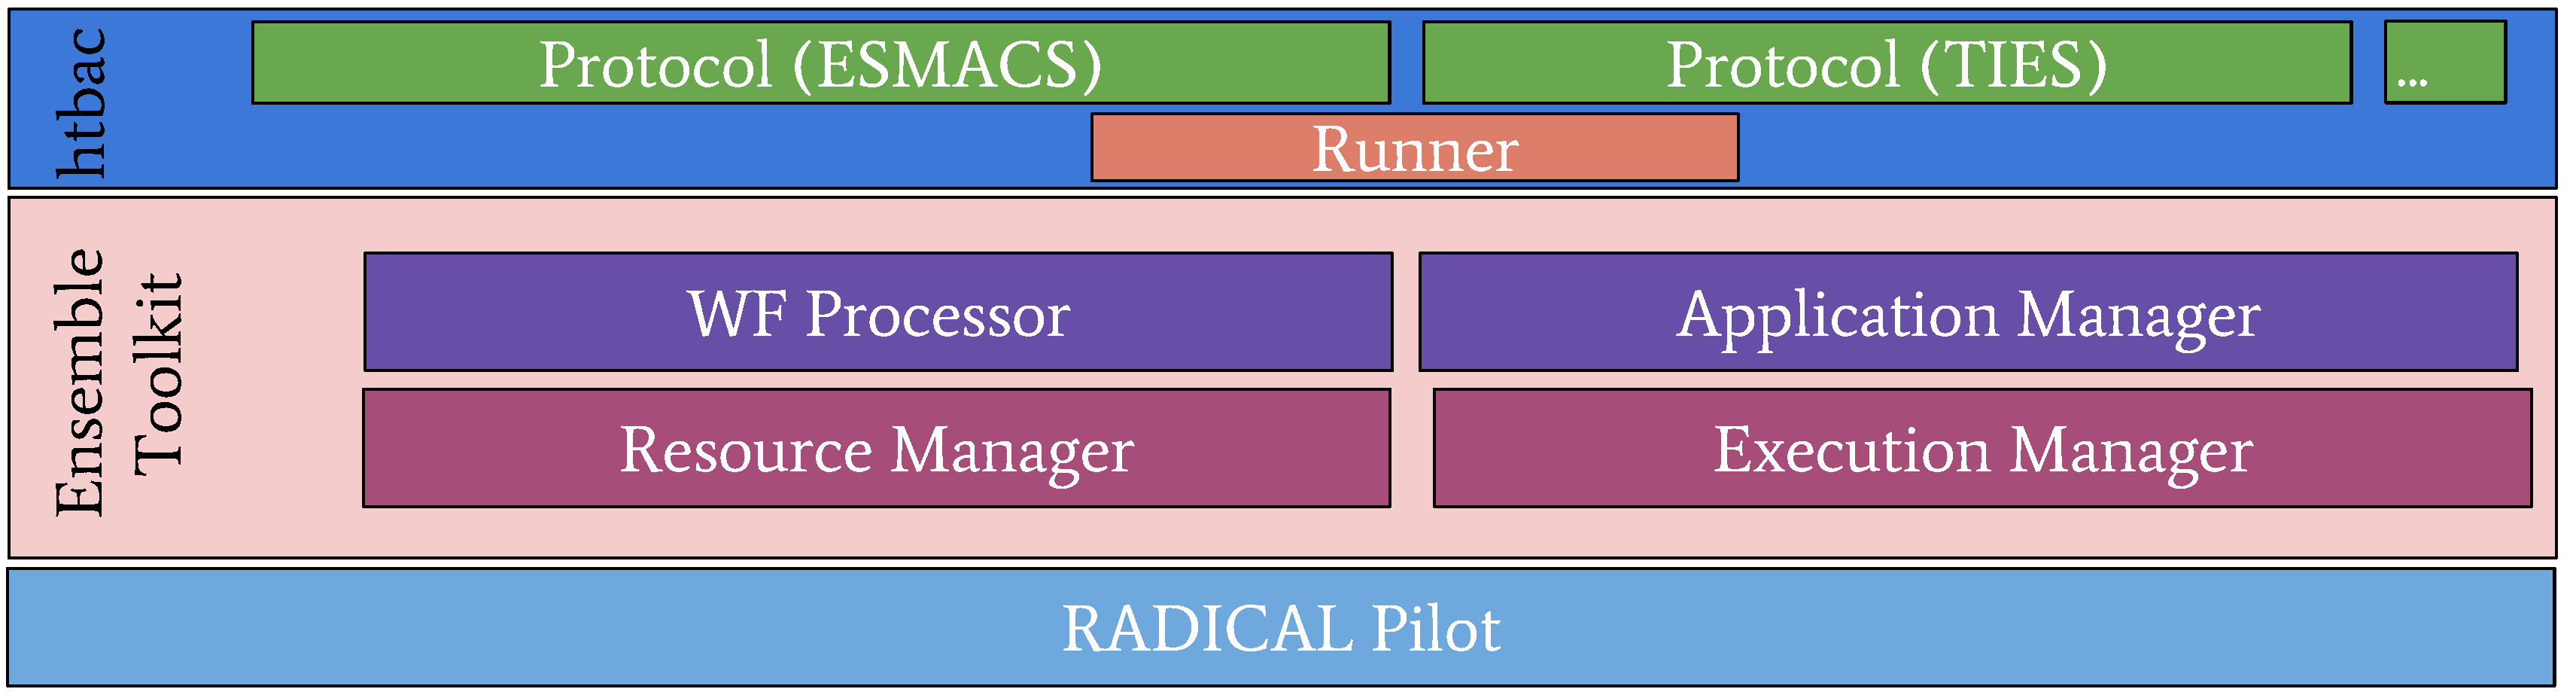
\includegraphics[width=\columnwidth]{figures/isc_htbac_integration_with_entk_RP.pdf}
  \caption{Mapping of flow between HTBAC, EnTK, and RP. The HTBAC API exposes the Protocol
  and Runner components. EnTK serves as the workflow execution system and
  by managing the workflow and workload. RADICAl-Pilot serves as the runtime system}
\label{fig:integration}
\end{figure}

	In our earlier work~\cite{dakka2017} we demonstrated how we applied the PST model to
implement the ESMACS protocol into an EnTK application. Here we expand upon this
work to further abstract the protocol implementation details and resource
information from the user. Domain scientists can leverage the generalization
of HTBAC and only need to define the ensemble parameters.

	HTBAC exposes two components \textbf{Runner Handle} and \textbf{Protocol}.
The \textbf{Runner} component is a container that implements the ESMACS 
and TIES into the EnTK PST model abstraction. The \textbf{Protocol} 
abstraction enables the user to select a protocol \textit{instance}, physical
system, number of replicas, core allocation per replica, and lambda 
windows (for alchemical pertubations). Currently the HTBAC abstraction provides
the ESMACS and TIES protocols. The user can scale protocol instances to study as
many physical systems as desired. The specification of protocols and 
their parameters are passed by the user to the \textbf{Runner Handle} which 
translates the request to EnTK. 

	In Section \ref{sec:related-work} we highlighted how an ensemble simulation 
approach can both aid sampling and provide improve uncertainty quantification 
for free energy calculations. Despite these crucial advantages, 
it remains non-trivial for field 
researchers to write biosimulation applications or protocols supporting 
multiple replica or multiple protocols in a given run. With HTBAC, this 
burden is minimized by specifying the number of replicas to the 
\textbf{Protocol} object, which determines the number of concurrent simulations. 
Moreover, the added ability to generate multiple protocols in a single interface 
enables the user to study a range of physical systems in a single run. 

%\jhanote{Is this specific to the TIES protocol or to the protocol class. Needs
%clarification.} 
%The same approach has been expanded to facilitate the creation of 
%sub-ensembles where the simulation configuration is altered programatically.
%An example of this is the implementation ofthe TIES protocol,
%where the user controls the $\lambda$ parameter values used in simulatios to 
%control which hybrid system states are sampled.

%A parameter, $\lambda \in [0, 1]$ is set for values between extremes and a
%simulation has to be run for every $\lambda$ value. The values form a function
%of energy and are integrated to obtain the desired results, the
%\emph{relative} binding free energy.


%\subsubsection{System}

%Systems This allows for multiple systems to be tested in the same
%\emph{single} run. A common scenario is the calculations of the binding
%affinity of a set of ligands with the same protein. System itself is just a
%collection of file paths pointing to descriptions of the system, like the
%system structure, topology etc. This class also provides the core/node
%requirments per single run, and reads some of the system descriptions from
%files to fill in the configuration settings.



%The Pipeline-Stage-Task (PST) framework developed by the Radical team
%(cite), and the Ensemble Toolkit (EnTK) built on top of it, offers a
%flexible way to express the molecular dynamics simulation workflows present
%in academia (cite) in terms of the radical pilot execution environment. Here
%we present a proposed mapping between the two (the PST and the MD layers)
%that is both simulation engine and protocol agnostic and allows for the
%compact expression of ensembles frequently used in binding affinity
%calculations.

%\subsection{Overview}

%The framework, called High Throughput Binding Affinity Calculator (HT-BAC),
%a python library, is made up of the following components: Workflow, Step,
%Ensembles and Simulation. These four object are all that is neccessary to
%describe the complex binding affinity caluculations in a generic way.

%\subsection{Workflow}

%The highest level abstraction is the Workflow. It is a container for the
%sequential units that are the simulation steps themselfs, and also contains
%meta-information about the job, like the resource description that the job
%will be running on, the total number of cores (nodes) required to fullfil
%the needs of the simulations and profiling mechanims to measure execution
%time.


% ---------------------------------------------------------------------------
%\jhanote{I don't these "description" should be subsections. Consider 
%"\paragraph{}"}

%\subsection{Step}

%\jhanote{what is a step? It is unclear to the reader. Is "step"  construct
%within HTBAC or is this just a description of the pipeline?}

%The workflow containts an ordered list of \emph{steps}. Steps give
%\jhanote{order?} orderd to the basic building blocks of binding affinity
%calculations. Usually they are (i) minimization (some form of local
%optimization of atom coordinates), (ii) heating, (iii) equilibration and (iv)
%production run.

%Additionally there is one or more steps of analysis at the end. The key
%point, is that these steps \emph{have} to be run consecutively, as they are
%dependent on the previous one. This is ensured by the \texttt{Stage} objects
%of EnTK\@. Each step has list of \texttt{Ensemble}s and a \texttt{Simulation}
%object.

% ---------------------------------------------------------------------------
%\subsection{Ensembles} 

%\jhanote{I'm not sure what we are trying to do here. We've just described
%the abstract/constructs in HTBAC to be protocols. Why are we regressing to
%presenting Ensembles as a construct in HTBAC, when they are a construct of
%EnTK?}

%Ensembles in HTBAC are a powerful construct that allows for extreme
%generalizations. At their core they are a nondestructively multi (forward)
%traversable \emph{iteratable}s. The underlying iterator yields a function that
%modifies a \texttt{Simulation} object to reflect the current state of the
%ensemble. This is similar to the iteratee construct, the only difference being
%that the function is applied to the \emph{same} data consecutively (as opossed
%to chunks of a stream of data).

%The Simulations are then generated for every Step based on what ensembles are
%attached to it. This is done by taking the \texttt{product} of all the
%ensembles, meaning that we go over every possible combination of ensemble
%states, and create a simulation from it. This is equivalent to an $n$ level
%deep for-loop, where $n$ is not known beforehand.

% ---------------------------------------------------------------------------
%\subsection{Simulation}

%Simulation is the lowest level building block. \jhanote{The use of building
%block for simulation will confuse the reader as it is overloading the term.
%Find alternative description.} It maps to the \texttt{Task} object in the PST
%model, and deals with executing the simulation engine, collecting input for
%it, and modifing the configuration of the simulation to reflect the ensembles
%that it is in.

%The main driver of a simulation is the configuration file. This file
%containts the specific settings of the Molecular Dynamics simulation,
%including the thermostat, barostat, constraints, long range force calculation
%methods and more. Some of the settings are general and apply to every
%simulation of a given step, but some are specific to the Ensemble that the
%simulation is in. After the ensemble modifies properties of the Simulation,
%these get propagated and written to the configuration file to be read by the
%executable.

% ---------------------------------------------------------------------------
%\subsection{Sandboxing}

%Sandboxing mechanims are built into the Radical stack for every layer. Each
%separate run has it's own sanbox, and inside each run, all the Tasks have
%their own sandbox too. This means that there is no unintented interference
%between Tasks, and data can be confidently analyised inside each sandbox.
%This mechanism also simplyfies the input data referencing, as the input in
%\emph{guaranteed} to be in the sandbox, and can be referenced relative to it.
%We recommend this sandboxing system for all simulations.

% ---------------------------------------------------------------------------
%\subsubsection{Data flow}

%while sandboxing offers a powerful way to separate the simulations, by the
%inherent nature of workflows, output data from one simulation is required as
%input for the next one. Simulation objects can find their previous
%couterparts by way of the ensemble that they are in. Then data is transfered
%via \textbf{copy-on-demand}, i.e. data is copied \emph{only} if it is known
%to be edited during execution, otherwise only a symbolic link is created to
%point to the original location of the file. This drasticly reduces the copy
%overhead, while still keeping the sandboxes separate.

% ---------------------------------------------------------------------------
\subsection{Adaptability}

%Once we tackle the barrier between the local workflow creation and the remote
%execution, new features become availble, and readily usable by scientists.
%Intraprotocol adaptability is one such new feature.

% ---------------------------------------------------------------------------
\subsubsection{Intraprotocol adaptability}

%while conceptually simple, tradiational execution patters used in academia
%makes this very hard. In HTBAC variables like replica size, specific lambda
%windows or simulatable system are settable on demand, the execution of which
%is automatically handeled by the library. To illustrate: a common scenario is
%the non adequate convergence of the statistical results after running a given
%number of replicas. In HTBAC the replica number can be changed, rerun and the
%results reevaluated. Additionally, logic can be written, to dynamically add
%more replicas until a given convergence tolerance has been reached.
